\setcounter{figure}{4}
\begin{figure}[H]
\centering
\par\smallskip\textbf{Panel S5, all views: partially reproduced}\par
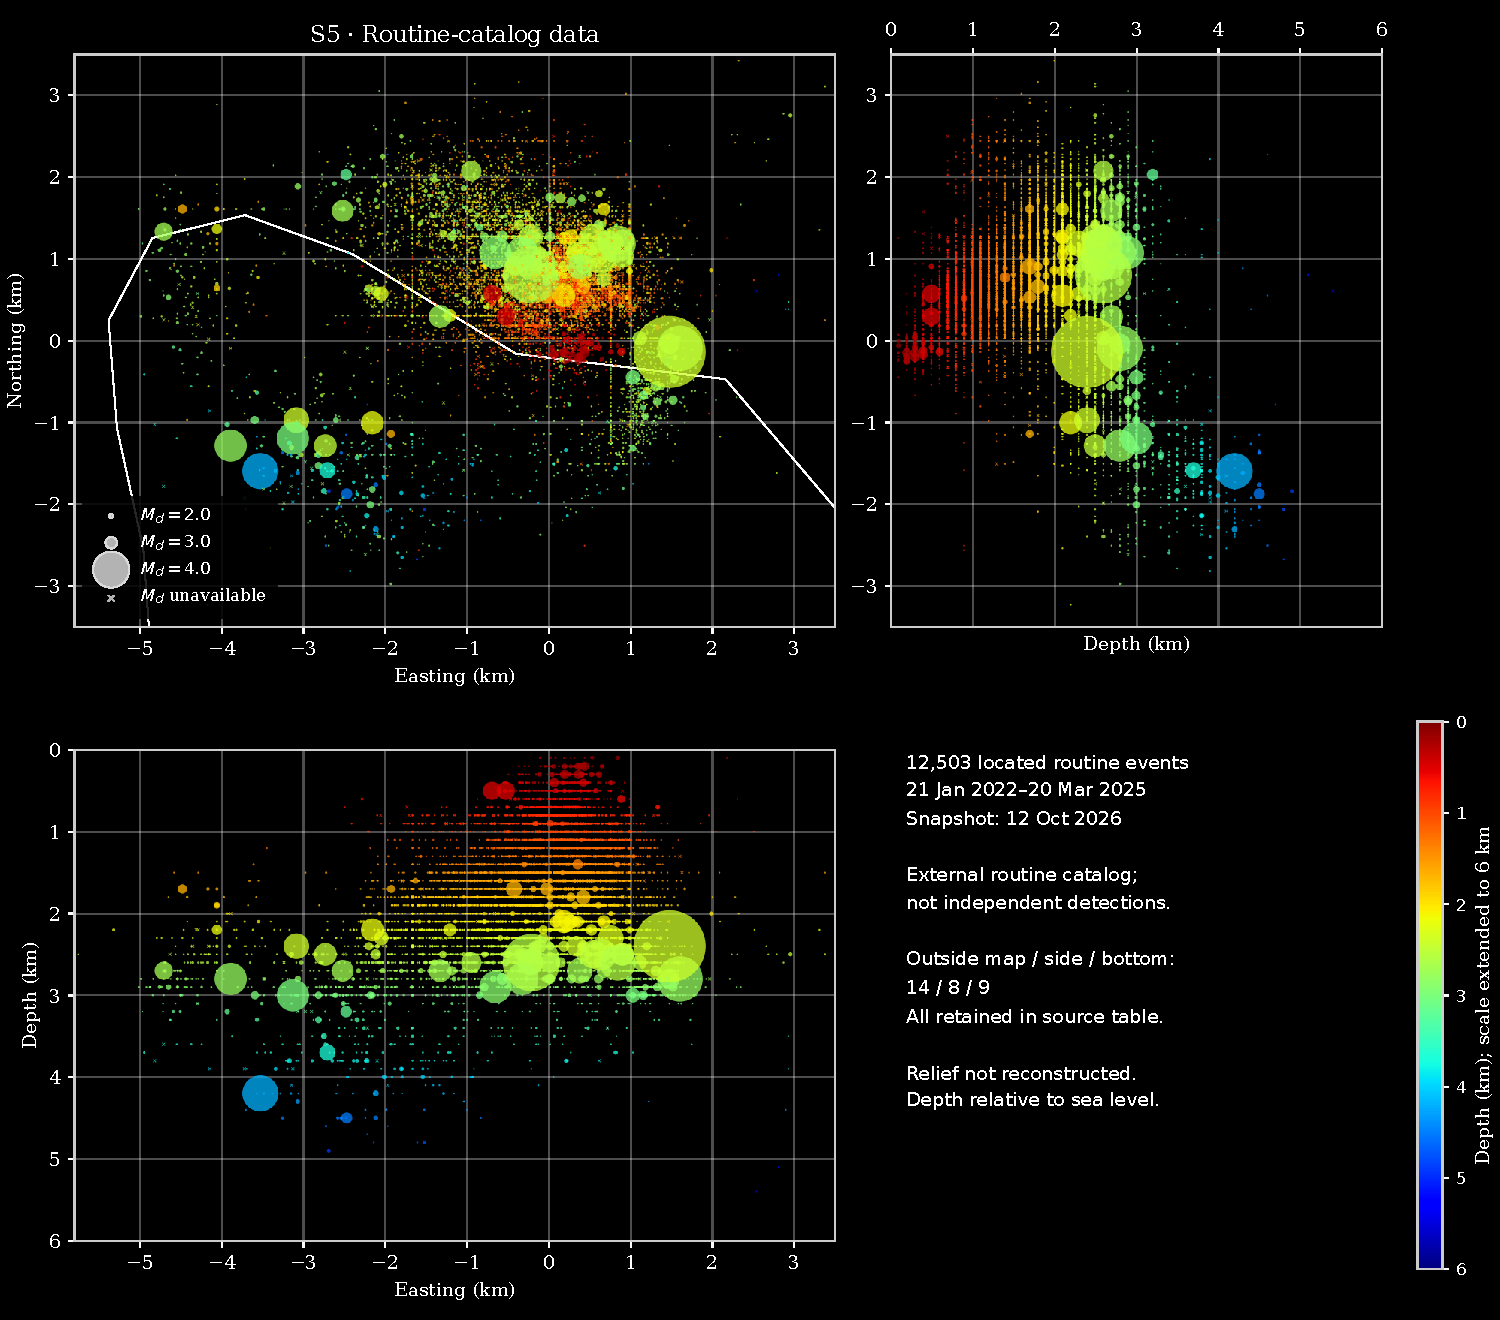
\includegraphics[width=.94\linewidth,height=.66\textheight,keepaspectratio]{figures/figure_S5_routine.pdf}
\caption{Routine-catalog locations. External routine-catalog data, independently selected and plotted: 12,503 located events, 21 January 2022--20 March 2025. This is 420 more than the published historical snapshot. No author-derived catalog is used to adjust that difference; these are not independent detections. Depth colors run red to blue on a dark background; the color scale extends to 6 km to include the observed range. Circle area includes an exponential Md term and a small visibility offset, an explicit display assumption; crosses indicate missing Md. Published pixels are not plotting inputs. The public source reports depths in 0.1 km steps; the resulting bands are not jittered or smoothed.}
\label{publication:S5}
\end{figure}
